\documentclass{jsarticle}
\usepackage[top=20truemm,bottom=20truemm,left=25truemm,right=25truemm]{geometry}
\usepackage{amsmath,ascmac,url,amsfonts,bm,here,algorithmic,algorithm,amsthm,color}
\usepackage[dvipdfmx]{graphicx}
\newcommand{\argmax}{\mathop{\rm argmax}\limits}
\newcommand{\argmin}{\mathop{\rm argmin}\limits} 
\newcommand{\expect}{\mathbb{E}} 
\newcommand{\trans}[1]{#1^{\top}}
\newcommand{\pdif}[2]{\frac{\partial#1}{\partial#2}}
\newcommand{\odif}[2]{\frac{\rm{d}#1}{\rm{d}#2}}
\makeatletter
  \def\@maketitle{
  \newpage\null
  \vskip 2em
    \mbox{}\hfill
    \begin{flushleft}
    \textbf{制御システム論分野研究会資料}
    \end{flushleft}
    \begin{flushright}
    {\lineskip .5em
      \begin{tabular}[t]{c}
        \@date \\
        \@author
      \end{tabular}\par}
        \end{flushright}
  \begin{center}
  \let\footnote\thanks
    {\LARGE \@title \par}
    \vskip 1.5em
  \end{center}
    \vskip 1em
  \par}
\makeatother
\title{\large{\bf{進捗報告 11.2}}}
\author{M2 竹内 維吹}
\date{\today}
\begin{document}
\maketitle


\section{はじめに}
近年, 機械学習分野で注目を集めているトピックとして強化学習というものがある. これは, ロボットなどが環境とのインタラクションを通じて, 最適な制御方策を見つけ出していくというものである. その中でも, 強化学習にニューラルネットワークを組み込んだ深層強化学習は, その適応能力の高さから多くの研究がなされている.しかしながら, 深層強化学習にはハイパーパラメータへの強い依存性など, 依然として課題点が多くまだまだ発展途上にある.\par
本稿では, 対象となる問題を最適セルフトリガー制御問題というものに絞り, 強化学習の課題点に対して有効な特性の調査に向けた準備を行う. まず,深層強化学習の基礎についての確認を行った後, 最適セルフトリガー制御問題を定式化し, その強化学習に特有の課題点を抽出する.最後に, その課題点の解決に向けた今後の展望についても簡単に述べる.

\section{方策勾配を用いた強化学習}
\subsection{強化学習の基礎知識}
マルコフ決定過程$M$を$M=\{S,A,T,d_0,r,\gamma\}$として与える。ここで$S,A$はそれぞれ状態,行動集合,~$T(s^{'}|s,a)$は状態遷移確率を表す.また$d_0,r(s,a),\gamma\in[0,1]$はそれぞれ初期状態分布, 報酬, 割引率を示す.\par
さて, 強化学習の目的は
\begin{equation}
	\pi^{*}=\argmax_{\pi}J(\pi) \label{purpose_of_rl}
\end{equation}を求めることである. ここで, 
\begin{align}
	V^{\pi}(s) &= \sum_{t=0}^{\infty}\gamma^tr(s_t, a_t)|_{a_t=\pi(s_t)}, s_0 = s\\
	J(\pi) &= \expect_{s_0\sim d_0}[V^{\pi}(s_0)]
\end{align}
であり,~$J(\pi), V^{\pi}(s)$をそれぞれ評価関数, (状態)価値関数とよぶ.\par
強化学習を解析するツールとして有用な関数として$Q$関数がある.
\begin{align}
	Q^{\pi}(s,a) &= r(s, a) + \gamma\sum_{t=1}^{\infty}\gamma^tr(s_t, a_t)|_{a_t=\pi(s_t)} \nonumber\\
			    &= r(s, a) + \gamma V^{\pi}(s^{\prime}) \label{Q_func}
\end{align}
式\eqref{Q_func} より,~$Q$関数は開始時刻において自由に行動$a$を選択して, 次ステップから方策$\pi$に従った時の価値を表す. したがって,~$Q$関数は行動価値関数という別名がある.

\subsection{方策反復法}
式\eqref{purpose_of_rl}を達成するためのアルゴリズムとして方策反復法というものがある.これは以下の2つのステップを繰り返すというものである.
\begin{enumerate}
	\item 方策評価: 行動価値関数$Q^{\pi}(s,a)$を求め(または, 近似す)る.
	\item 方策改善: 求めた$Q^{\pi}(s,a)$に従って, ~$\pi(s)=\argmax_aQ^{\pi}(s,a)$と方策を更新する.
\end{enumerate}
以上の2ステップを繰り返すことで最適方策$\pi^{*}$が得られることが知られている.(方策改善定理)

\subsection{状態空間, 行動空間の特性に合わせたアルゴリズム}
状態空間も行動空間も離散値をとる場合,~$Q^{\pi}(s,a)$をテーブルに保存しておくことで, 前節で登場した$\pi(s)=\argmax_aQ^{\pi}(s,a)$を容易に求めることができる.\par
では, 状態空間が連続値の場合はどうか. 状態$s$が無限種類の値をとることになるため, テーブルに保存することができない. そこでMinhら\cite{DQN}は, $Q^{\pi}(s,a)$をニューラルネットワークを用いてパラメトライズして近似するアプローチをとった. ここでも, 行動空間は離散であるため$\argmax_aQ^{\pi}(s,a)$を求めることは可能である.\par
最後に, 状態空間も行動空間も連続値である場合は$\argmax_aQ^{\pi}(s,a)$を求めるのに膨大なコストがかかるという問題点がある. したがって, これまでは方策$\pi$は$Q$関数によって定めていたが, 両空間が連続値の場合にはこのアプローチはとれない. そこで, 方策関数も独立に$\pi_{\theta}$のようにパラメトライズした関数として用意し,~パラメータ$\theta$を勾配法などで更新する手法が取られることが多い.

\subsection{方策勾配による方策関数のパラメータの更新}
Silverら\cite{DPG}は, 方策が$\pi(s)$のように決定論的に定めるものとして与えた場合に, 評価関数$J(\pi_{\theta})$に対する勾配を計算する手法を発見した. この勾配は決定論的方策勾配(DPG:Deterministic Policy Gradient)とよばれ, 以下のように計算することができる.
\begin{align}
	\nabla_{\theta}J(\pi_{\theta}) &= \expect_{s\sim\rho^{\pi}}[
	\nabla_{\theta}\pi_{\theta}(s)\nabla_{a}Q^{\pi_{\theta}}(s, a)|_{a=\pi_{\theta}(s)}] \label{true_pg} 
\end{align}
ただし, 
\begin{equation}
	\rho^{\pi}(s) = \int_{S}\sum_{t=0}^{\infty}\gamma^td_0(s_0)\textrm{Pr}(s_0\to s, t,  \pi)\textrm{d}s_0
\end{equation}
を割引分布という.\par
この方策勾配を深層強化学習の枠組みに取り入れたアルゴリズムがDDPG(Deep DPG)\cite{DDPG}である.これはActor-Critic構造を採用しており,~$Q^{\pi_{\theta}}$を近似するcriticネットワーク$Q(s,a|\omega)$と,方策$\pi$を表現するactorネットワーク$\pi(s|\theta)=\pi_{\theta}$をそれぞれ学習する手法である. 以下に,この近似勾配を用いたactorとcriticの更新アルゴリズムを記す.\par
DDPGはミニバッチ学習を用いる. 過去の経験データ$(s_t, a_t, r_t, s_{t+1})$を保存しておき, その中から$N$個のデータを取り出し(ミニバッチ, $E$と記載する),そのデータ集合に対する最適化を行う. まず, criticの更新から記す.~criticの目的は$Q^{\pi}$を近似することである.~$Q$関数は式\eqref{Q_func}のように分解することが可能で有るため,~$Q(s,a|\omega)$もこれを満たすように更新すればよい.そのためにTD(Temporal Difference)誤差
\begin{equation}
	\textrm{TD} = Q(s,a|\omega) - \{r(s,a)+\gamma Q(s,\pi(s)|\omega)\}
\end{equation}
が最小となる方向に$\omega$を更新する. 全ての$(s,a)$についてこれを一度に行うことはできないので, 作成したミニバッチ$E$に対する平均二乗誤差
\begin{equation}
	Loss = \frac{1}{N}\sum_{s\in E} \textrm{TD}^2
\end{equation}
をLoss関数として, このLoss関数を減らすようにアルゴリズムを働かせる. \par
さて, 上記のcriticの更新方法は教師あり学習そのものである. 従ってミニバッチに含まれるデータはi.i.d.であることが要求される. もしミニバッチ$E$がエージェントが経験した直近の$N$ステップのデータを用いると, これらは独立ではなくなってしまう. 従って, エージェントは環境とのインタラクションによって得られた経験データをexperience replayに保存しておき, そこから無作為に$N$このデータを選びとる手法でデータの分散を上げている.\par
次にactorの更新を記す.~actorは方策関数$\pi(s)$を表現するものであり, パラメータの更新には方策勾配を用いる.ただし,~DDPGでは式\eqref{true_pg}のように正しい$Q$関数を用いることができないので, 
\begin{equation}
	\expect_{s\sim\rho^{\pi}}[\nabla_{\theta}\pi_{\theta}(s)\nabla_{a}Q(s, a|\omega)|_{a=\pi_{\theta}(s)}] \simeq \nabla_{\theta}J(\pi_{\theta}) 
\end{equation}
のようにcriticネットワークを用いて近似した方策勾配を用いる. さらに, 期待値に関して, 
\begin{equation}
	\expect_{s\sim\rho^{\pi}}[\nabla_{\theta}\pi_{\theta}(s)\nabla_{a}Q(s, a|\omega)|_{a=\pi_{\theta}(s)}] \simeq \frac{1}{N}\sum_{s\in E}[\nabla_{\theta}\pi_{\theta}(s)\nabla_{a}Q(s, a|\omega)|_{a=\pi_{\theta}(s)}]
\end{equation}
という近似も行っている. 従って, この近似勾配$g=\frac{1}{N}\sum_{s\in E}[\nabla_{\theta}\pi_{\theta}(s)\nabla_{a}Q(s, a|\omega)|_{a=\pi_{\theta}(s)}]$はcriticの近似精度とミニバッチの分布によって大きく性能を落としてしまう可能性があり, 大きな問題点であると言える.

\section{最適セルフトリガー制御問題に対する強化学習}
\subsection{セルフトリガー制御}
図\ref{image}のような制御系を考える.
\begin{figure}[h]
	\centering
 	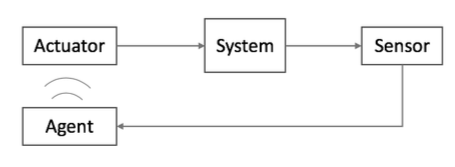
\includegraphics[width=10cm]{event.png}
 	\caption{制御系} \label{image}
\end{figure}\par
これに対するフィードバック制御を考える. 状態変数$s$を観測してアクチュエータに入力信号を送信することを「インタラクション」と呼ぶと,セルフトリガー制御では, 連続的なインタラクションは行わずに, 次のインタラクションを何秒後に行うかをエージェントが決定する. それを数式上で表すため, エージェントの制御則$\pi(s)$は2つの要素からなるベクトル値関数であるとし, 1つ目の要素はアクチュエータに送信する入力$a$,~2つ目の要素は次にインタラクションを行うまでの時間間隔$\tau~(s:秒)$を表すものとする.また, 次のインタラクションを行う時刻までは1つ前のインタラクションで送信した入力$a$を加え続けるものとする(ZOH制御).

\subsection{最適セルフトリガー制御}
最適なセルフトリガー制御則$\pi^{*}$を, 以下のように定義する. 
\begin{align}
	\pi^{*} &= \argmax_{\pi}J(\pi) \label{optimal_policy}\\
	J(\pi) &= \expect_{s_0\in d_0}[V^{\pi}(s_0)] \\
	% V^{\pi}(s_0) &= \sum_{i=0}^{\infty} \gamma^i\{-s_i^{\top}Qs_i-\pi_1(s_i)^{\top}R\pi_1(s_i)+\lambda \pi_2(s_i)\} \\
	V^{\pi}(s_0) &= \sum_{i=0}^{\infty} \gamma^i r^{\pi}_i \label{value} \\
	r^{\pi}_i &= -\int_{T_i}^{T_{i+1}}s(t)^{\top}Qs(t)\textrm{d}t +\tau_ia_i^{\top}Ra_i + \lambda \tau_i, ~T_i = \sum_{l=0}^{i} \tau_l \label{reward}
\end{align}
ここで, $i$はインタラクションの回数を示し, $a_i, \tau_i$はそれぞれ$i$回目のインタラクションでの方策$\pi$の出力であるとする. \par
さて, 一般的に強化学習では, 1ステップ1ステップの行動の良し悪しを評価して方策を更新していく. 
インタラクションとインタラクションの間の区間を「インターバル」と呼ぶと, 式(\ref{value})より, この問題は各インターバルを1ステップとした強化学習問題であると考えることができる. \par

\section{数値実験による課題点の抽出}
上記の問題は, 一般的な強化学習のフレームワークにそのまま落とし込むことができるため, 数値実験を行うことが可能である. 数値実験の結果を通して, 最適セルフトリガー制御の強化学習にどのような課題点があるのかを考察していく.\par
実験環境はOpen-AI Gymのpendulumで, 初期状態が$\theta\sim N(0, \pi), \dot{\theta}\sim U(-\pi,\pi)$となるような環境で行った. またreplay bufferの分散を上げるため,~10秒間の制御を1エピソードと定義し, エピソードを重ねることで経験データを増やしていく. また, pendulumは以下のようなダイナミクスに従っており入力アフィン系の非線型システムである.
\begin{equation}
	\odif{}{t}\begin{pmatrix}\theta \\ \dot{\theta}\end{pmatrix} = 
		\begin{pmatrix}\dot{\theta} \\ \frac{3g}{2l}\sin{\theta} + \frac{3}{ml^2}a \end{pmatrix} \label{pendulum}
\end{equation}

\subsection{初期方策}
学習の初期方策として
\begin{align}
\begin{cases}
	a(s)=a_{0.001}^{*}(s)\\
	\tau(s)=0.001
\end{cases} \label{pi_init}
\end{align}
とする方策$\pi_{\rm{init}}$を用いる.ただし, $a_{0.001}^{*}(s)$はシステム\eqref{pendulum}を,離散化幅$\delta_t=0.001$として離散化したシステムを原点付近で安定化する制御則として与える.

\subsection{学習の様子からみる勾配法の進捗の確認}
式\eqref{reward}より, $\tau$を大きくするモチベーションは$\lambda$に大きく依存するため, それを様々な値にすることでど学習過程にどのような変化が見られるのかを確認してみた. ここでは,~$\lambda$を$0.05, 0.5, 5, 50$に設定し, それぞれ3回, 200000ステップ(インタラクションの回数)の強化学習を行った. また,~$\tau$は$0.001\sim0.1$の範囲に制限している.\par
まずそれぞれの学習タスクの中で, 1エピソードの間の$\tau$の平均値の変化を見てみる.\par
\begin{figure}[h]
	\centering
 	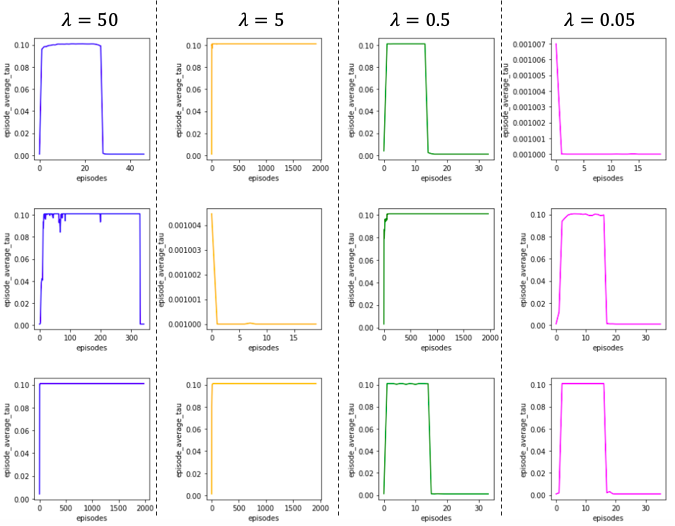
\includegraphics[width=14cm]{tau_exp_ave.png}
 	\caption{学習を通しての$\tau$の変化} \label{average_tau}
\end{figure}\par
ここで注意したいのは, $\tau$によって200000回のインタラクションに含まれるエピソード数が異なる点である. 例えば$\tau$の学習が進まずにずっと$\tau=0.001$であった場合, 10秒間の制御の間には10000回のインタラクションが行われる. したがって200000回のインタラクションの間には20エピソードしか含まれない. 逆に, 初期から$\tau$の学習が進み$\tau=0.1$となることが増えてくると, エピソード数は増えてくる. 図\ref{average_tau}の$x$軸の範囲が異なるのはそのためである. \par
図\ref{average_tau}をみると, 勾配法の収束は(200000ステップの間は)見ることができない. このことから, 近似勾配$g=\frac{1}{N}\sum_{s\in E}[\nabla_{\theta}\pi_{\theta}(s)\nabla_{a}Q(s, a|\omega)|_{a=\pi_{\theta}(s)}]$のノルムの200000ステップの間の変化を見てみる. 
\begin{figure}[h]
	\centering
 	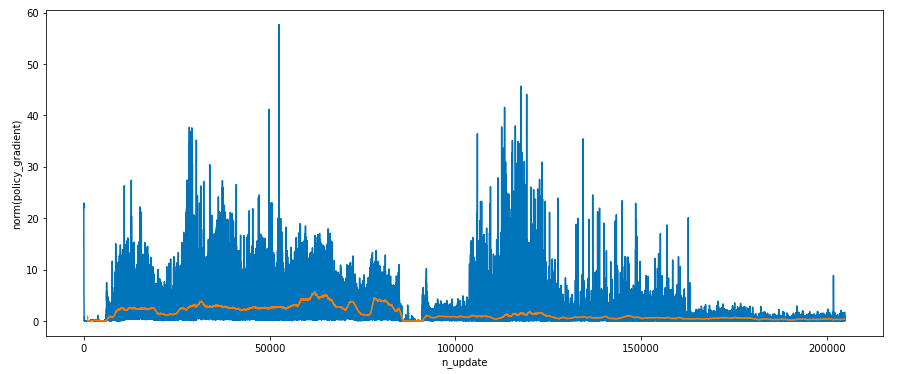
\includegraphics[width=14cm]{gradient_log.png}
 	\caption{学習を通しての$\|g\|$の変化} \label{gradient_log}
\end{figure}\par
図\ref{gradient_log}をみると, 勾配のノルム$\|g\|$は収束していない. また, 100000ステップあたりで突然大きな勾配になっていることがわかる. 以下では, このような問題が生じている原因について検討していく.

\subsection{勾配法が収束しない原因の検討}
2.4節で示したDDPGのアルゴリズム自体の問題点以外に, 前節の問題点の原因となる候補を考察する. \par
まず1つ目として,~$Q$関数の近似が正しく行えていないことが考えられる. actorの更新には
\begin{equation*}
	g=\frac{1}{N}\sum_{s\in E}[\nabla_{\theta}\pi_{\theta}(s)\nabla_{a}Q(s, a|\omega)|_{a=\pi_{\theta}(s)}]
\end{equation*}
が用いられるため,~$Q$関数の近似精度は必要不可欠である. しかしながら, DDPGでは各ステップにおける方策$\pi_{\theta_k}$に対する$Q^{\pi_{\theta_k}}$の学習が収束する前に次ステップに進む場合があり, この場合は間違った方向にactorの更新がなされることになる.\par

2つ目に, 正しい方策勾配\eqref{true_pg}がパラメータ空間上で非常に変化が激しい領域がある可能性があることである. 図\ref{gradient_log}をみると, 一度近似勾配$g$のノルムが小さくなった後再び大きくなっている. もしノルムが小さくなっているステップ周辺での$Q$関数が正しく近似されており, replay buffer の分布が$\rho^{\pi_{\theta_k}}$に近いのならば,用いられた勾配は正しい値となる.これが急激に大きくなっているのなら, その場合のステップサイズを小さくしておく必要がある. また, 方策が大きく変化するとcriticのパラメータ$\omega$の再学習も必要となり, 1つ目の問題点の影響を受けることになる.\par

\section{課題点抽出}
前節で行った考察より, まず方策勾配を解析的に計算してパラメータ空間上で急峻な変化をもつ構造かどうかを確認する. もし予想の通りであれば, そのパラメータ付近で意図的にステップサイズを小さくする手法を考案する.逆に, 急峻となる構造でないのならば,~replay bufferのデータの分布に問題があるということになり, システムとのインタラクション方法について考察する必要がある.\par
方策勾配の解析的な計算についてであるが, 図\ref{gradient_log}に見られた問題点は, 最適セルフトリガー制御の強化学習に特有の特徴であったため,~$\nabla_{\theta^a}J(\pi_{\theta}),~\nabla_{\theta_{\tau}}J(\pi_{\theta})$についてそれぞれ計算を行いたいと考えている. \par

\section{方策勾配の大きさによる, 入力信号$a$と通信間隔$\tau$の学習率の考察}
図\ref{split_NN}のようにactorネットワークを, ~$a(s)$と$\tau(s)$を分離したモデルとして用いる. 
\begin{figure}[h]
	\centering
 	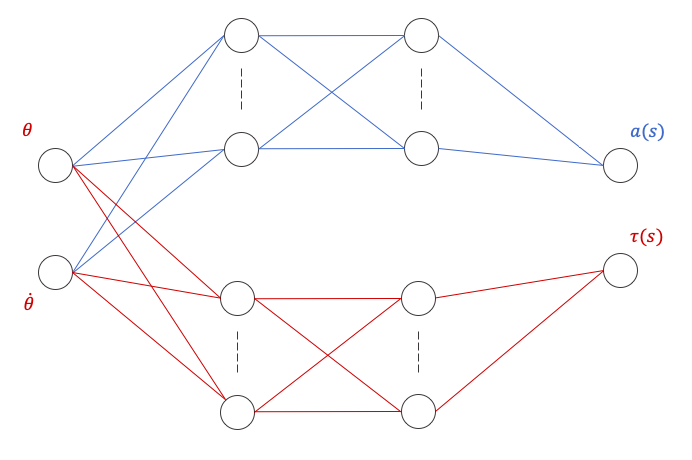
\includegraphics[width=10cm]{split_NN.png}
 	\caption{actorネットワーク} \label{split_NN}
\end{figure}\\
actorネットワークの全パラメータを$\theta^{\mu}$,~$a(s)$と$\tau(s)$を表す部分ネットワークのパラメータをそれぞれ$\theta^a, \theta^{\tau}$とする.このとき, 方策勾配$\nabla_{\theta^{\mu}}J(\theta^{\mu})$もそれぞれのパラメータが表す部分を分けて, $\nabla_{\theta^a}J(\theta^{\mu}), \nabla_{\theta^{\tau}}J(\theta^{\mu})$としたとき, パラメータの更新則は以下のようになる.
\begin{equation}
	\theta^{\mu}\gets \theta^{\mu} - \alpha_a\nabla_{\theta^a}J(\theta^{\mu}) - \alpha_{\tau}\nabla_{\theta^{\tau}}J(\theta^{\mu})
\end{equation}
研究の1つの成果物として,~$\alpha_a, \alpha_{\tau}$の理論的な大きさの設定方法について言及できればと考えている.そのため, 勾配$\nabla_{\theta^a}J(\theta^{\mu}), \nabla_{\theta^{\tau}}J(\theta^{\mu})$の大きさをそれぞれみてみる.~($\theta^{\tau}, \theta^{a}$はそれぞれ同じ長さのパラメータベクトルにしています.)\par
6.1節でcriticが収束した$\pi_1, \pi_2$について, その方策勾配$\nabla_{\theta^a}J(\theta^{\mu}), \nabla_{\theta^{\tau}}J(\theta^{\mu})$のノルムを計算すると, $\pi_1$での値は
\begin{align}
	\|\nabla_{\theta^a}J(\theta^{\mu})\| &= 66.70076 \\
	\|\nabla_{\theta^{\tau}}J(\theta^{\mu})\| &= 8.730332e-05
\end{align}
$\pi_2$での値は,
\begin{align}
	\|\nabla_{\theta^a}J(\theta^{\mu})\| &= 1.9210727 \\
	\|\nabla_{\theta^{\tau}}J(\theta^{\mu})\| &= 4.414095e-05
\end{align}
となった. このことから,~$\theta^{\tau}$の微小変化が$J$に与える影響が非常に小さいことが見てとれる. \par

\section{2つのパラメータに関する方策勾配の考察}
前節で行った検証により倒立振子の場合には, ~actorを表現する2つのニューラルネットワークのパラメータに関する方策勾配$\nabla_{\theta^a}J(\theta^{\mu}), \nabla_{\theta^{\tau}}J(\theta^{\mu})$の大きさがかなり異なっていた. このことから, 制御対象に関するどのような前提があれば$\|\nabla_{\theta^a}J(\theta^{\mu})\|>\|\nabla_{\theta^{\tau}}J(\theta^{\mu})\|$となるのかを考えてみる.\par
評価関数$J(\theta^{\mu})=\expect_{s_0\sim d_0}[V^{\theta^{\mu}}(s_0)]$であることから$\nabla_{\theta^{\mu}}J(\theta^{\mu})=\int_{S}d_0(s)\nabla_{\theta^{\mu}}V^{\theta^{\mu}}(s)\textrm{d}s$なので, まず$\nabla_{\theta^{\mu}}V^{\theta^{\mu}}(s)$について詳しくみていく. 価値関数$V^{\theta^{\mu}}(s)$の(一般的な)性質から, 
\begin{equation}
	\nabla_{\theta^{\mu}}V^{\theta^{\mu}}(s) = \nabla_{\theta^{\mu}}[r(s, \mu(s|\theta^{\mu}))+\gamma V^{\theta^{\mu}}(s^{\prime})]
\end{equation}
微分のchain~ruleより,
\begin{align}
	\nabla_{\theta^{\mu}}V^{\theta^{\mu}}(s) &= \nabla_{\theta^{\mu}}\mu(s|\theta^{\mu})\nabla_ur(s, u)|_{u=\mu(s|\theta^{\mu})}\nonumber\\
	&+\gamma\int_{S}\nabla_{\theta^{\mu}}\mu(s|\theta^{\mu})\nabla_{u}\textrm{Pr}(s^{\prime}|s, u)|_{u=\mu(s|\theta^{\mu})}V^{\theta^{\mu}}(s^{\prime})\textrm{d}s^{\prime}\nonumber\\
	&+\gamma\int_{S}\textrm{Pr}(s^{\prime}|s, \mu(s))\nabla_{\theta^{\mu}}V^{\theta^{\mu}}(s^{\prime})\textrm{d}s^{\prime} \label{recurrence}
\end{align}
となる(ただし,~$u=[a,\tau$]). この式は微分するパラメータをactor全体のパラメータ$\theta^{\mu}$ではなく,入力信号$a$, 通信間隔$\tau$のネットワークのパラメータのみに絞った場合にも同じような式が成り立つはずである. つまり,
\begin{align}
	\nabla_{\theta^{a}}V^{\theta^{\mu}}(s) &= \nabla_{\theta^{a}}\mu(s|\theta^{\mu})\nabla_{a}r(s, u)|_{u=\mu(s|\theta^{\mu})}\nonumber\\
	&+\gamma\int_{S}\nabla_{\theta^{a}}\mu(s|\theta^{\mu})\nabla_{a}\textrm{Pr}(s^{\prime}|s, u)|_{u=\mu(s|\theta^{\mu})}V^{\theta^{\mu}}(s^{\prime})\textrm{d}s^{\prime}\nonumber\\
	&+\gamma\int_{S}\textrm{Pr}(s^{\prime}|s, \mu(s))\nabla_{\theta^{a}}V^{\theta^{\mu}}(s^{\prime})\textrm{d}s^{\prime} \label{recurrence_a}
\end{align}
\begin{align}
	\nabla_{\theta^{\tau}}V^{\theta^{\mu}}(s) &= \nabla_{\theta^{\tau}}\mu(s|\theta^{\mu})\nabla_{\tau}r(s, u)|_{u=\mu(s|\theta^{\mu})}\nonumber\\
	&+\gamma\int_{S}\nabla_{\theta^{\tau}}\mu(s|\theta^{\tau})\nabla_{\tau}\textrm{Pr}(s^{\prime}|s, u)|_{u=\mu(s|\theta^{\mu})}V^{\theta^{\mu}}(s^{\prime})\textrm{d}s^{\prime}\nonumber\\
	&+\gamma\int_{S}\textrm{Pr}(s^{\prime}|s, \mu(s))\nabla_{\theta^{\tau}}V^{\theta^{\mu}}(s^{\prime})\textrm{d}s^{\prime} \label{recurrence_tau}
\end{align}が成り立つ.以下$\theta_{\tau}, \theta_a$の両方に成り立つ議論をする場合に, 便宜上$\theta$を用いることとする.  \par
システム\eqref{continuous}は確定系なので, 
\begin{equation}
	s^{\prime} = s + \int_{0}^{\tau(s)}(f(t)+g(t)a(s))\textrm{d}t
\end{equation}
と定まり, 各漸化式の第3項目は
\begin{equation}
	\int_{S}\textrm{Pr}(s^{\prime}|s, \mu(s))\nabla_{\theta}V^{\theta^{\mu}}(s^{\prime})\textrm{d}s^{\prime}=\nabla_{\theta}V^{\theta^{\mu}}(s + \int_{0}^{\tau(s)}(f(t)+g(t)a(s))\textrm{d}t)
\end{equation}
となる.\par
またシステムと方策$\pi(s)$が確定的であるので, 全インターバルの開始時刻での状態は, 初期状態を引数とする関数で書け, $s^{(n)}(s)$と表記する. 同じく, 漸化式の第1,2項目までの和も確定的であり, $k^{(n)}(s)$とすれば, 
\begin{align}
	\nabla_{\theta}V^{\theta^{\mu}}(s) = \sum_{n=0}^{\infty} \gamma^{i}k^{(n)}(s)
\end{align}
となるため, $k^{(n)}(s)$を解析的に表現できれば, 価値関数の勾配を解析的に書けそうである.

\subsection{注意}
$\nabla_{\theta^{\tau}}\mu(s|\theta^{\mu})$,~$\nabla_{\theta^{a}}\mu(s|\theta^{\mu})$に関しては, ニューラルネットワークモデルの設定にしか依存しないものなので, 今回は特段着目しない.

\subsection{各ステップの報酬のパラメータ勾配}
初めに, 漸化式\eqref{recurrence_tau}の右辺第1項に関して考察する.~$T$を各インターバルの開始時刻だとすると, 
\begin{align}
	\nabla_{\tau}r(s, u)|_{u=\mu(s|\theta^{\mu})} &= -\nabla_{\tau}\int_{T}^{T+\tau} s(t)^{\top}Qs(t)\textrm{d}t - \nabla_{\tau}(\tau a^{\top}Ra) + \nabla_{\tau}(\lambda\tau) \nonumber\\
	&= -\nabla_{\tau}\int_{0}^{\tau} s(t+T)^{\top}Qs(t+T)\textrm{d}t - a^{\top}Ra + \lambda \nonumber\\
	&= - s(\tau+T)^{\top}Qs(\tau+T) - a^{\top}Ra + \lambda \label{reward_tau_gradient}
\end{align}
となる. ただし, 
\begin{equation}
	s(t+T) = s(T) + \int_{0}^{t} (f(l+T)+g(l+T)a(T))\textrm{d}l \label{solution}
\end{equation}
であることを注意しておく.
\par
次に, 漸化式\eqref{recurrence_a}の右辺第1項に関して考察する. 
\begin{align}
	\nabla_{a}r(s, u)|_{u=\mu(s|\theta^{\mu})} &= -\nabla_{a}\int_{T}^{T+\tau} s(t)^{\top}Qs(t)\textrm{d}t - \nabla_{a}(\tau a^{\top}Ra) + \nabla_{a}(\lambda\tau) \nonumber\\
	&= -\nabla_{a}\int_{0}^{\tau} s(t+T)^{\top}Qs(t+T)\textrm{d}t - \tau Ra \nonumber\\
	&= -\int_{0}^{\tau} (\pdif{s(t+T)}{a}^{\top}Qs(t+T)+s(t+T)^{\top}Q\pdif{s(t+T)}{a})\textrm{d}t - \tau Ra \nonumber \\
	&= -2\int_{0}^{\tau} s(t+T)^{\top}Q\pdif{s(t+T)}{a}\textrm{d}t - \tau Ra~(∵Q:対称)
\end{align}
式\eqref{solution}より, 
\begin{align}
	\pdif{s(t+T)}{a} &= \pdif{}{a}\int_{0}^{t} (f(l+T)+g(l+T)a)\textrm{d}l \nonumber \\
	&= \int_{0}^{t} g(l+T)\textrm{d}l
\end{align}
なので, 
\begin{equation}
	\nabla_{a}r(s, u)|_{u=\mu(s|\theta^{\mu})} = -2\int_{0}^{\tau}s(t+T)^{\top}Q\left\{\int_{0}^{t}g(l+T)\textrm{d}l\right\}\textrm{d}t - \tau Ra \label{reward_a_gradient}
\end{equation}
と表せる.したがって, インターバルの開始状態$s(T)$と,~$u=\mu(s|\theta^{\mu})$がわかれば各インターバルにおけるステップ報酬の勾配の比較は可能である.\par
最後に, 各インターバルの開始時刻での状態は
\begin{equation}
	s^{(n)}(s) = s^{(0)}(s) + \sum_{i=0}^{n−1}\int_{T_i}^{T_i + \tau(s^{(i)}(s))}(f(T_i+t)+g(T_i+t)a(s^{(i)}(s)))\textrm{d}t
\end{equation}
と書けるため, 式\eqref{reward_tau_gradient}, \eqref{reward_a_gradient}に代入すれば全ステップでの$r$の勾配は, 関数$V$の引数$s$の関数として表せる. ただし,~$T_i = \sum_{i=0}^{n-1}\tau(s^{(i)}(s))$である. 


\section{勾配計算}
評価関数$J(\theta^{\mu})=\expect_{s_0\sim d_0}[V^{\theta^{\mu}}(s_0)]$であることから$\nabla_{\theta^{\mu}}J(\theta^{\mu})=\int_{S}d_0(s)\nabla_{\theta^{\mu}}V^{\theta^{\mu}}(s)\textrm{d}s$なので, まず$\nabla_{\theta^{\mu}}V^{\theta^{\mu}}(s_0)$について詳しくみていく. 価値関数$V^{\theta^{\mu}}(s)$の定義から, 
\begin{equation}
	\nabla_{\theta^{\pi}}V^{\theta^{\pi}}(s_0) = \nabla_{\theta^{\pi}}\sum_{i=0}^{\infty}\gamma^{i}r(s_i, \pi(s_i|\theta^{\pi}))\label{first_step}
\end{equation}
と書ける. ただし$s_i$は$i$回目のインタラクションの開始時刻における状態変数の値である. もちろん全ての$i$に対して, これは初期状態$s_0$, パラメータ$\theta^{\tau}, \theta^a$に対して一意に定まる量であるので, 
\begin{equation}
	s_i = \mathcal{S}(s_0, \theta^{\tau}, \theta^{a}, i)
\end{equation}
のように関数$\mathcal{S}$を用いて表す. また, 各ステップ内での状態変化を記述するために関数$\chi_i(t)$を導入する. これはステップの開始時刻を0と見た時の, そのステップの中での状態変化を表す.したがって$\chi_i(0) = s_i, \chi_i(\tau(s_i))=\chi_{i+1}(0)=s_{i+1}$となる. これを用いると, 各ステップの開始時刻での状態$s_i$は次のように書ける.
\begin{equation}
	\mathcal{S}(s_0, \theta^{\tau}, \theta^{a}, i) = s_0 + \sum_{t=0}^{i}\int_{0}^{\tau(\mathcal{S}(s_0, \theta^{\tau}, \theta^{a}, t)|\theta^{\tau})}\left\{f(\chi_t(l))+g(\chi_t(l))a(\mathcal{S}(s_0, \theta^{\tau}, \theta^{a}, t)|\theta^a)\right\}\textrm{d}l \label{step_state}
\end{equation}
さて, 式\eqref{first_step}に話を戻し, もう少し計算を進めていく. ここでは微分を$\theta^{\pi}$の一部のパラメータ($\theta$を用いて表す)で行う.
\begin{align}
	\nabla_{\theta}V^{\theta^{\pi}}(s_0) &= \nabla_{\theta}\sum_{i=0}^{\infty}\gamma^{i}r(\mathcal{S}(s_0, \theta^{\tau}, \theta^{a}, i), \pi(\mathcal{S}(s_0, \theta^{\tau}, \theta^{a}, i)|\theta^{\tau}, \theta^a)) \\
	&= \sum_{i=0}^{\infty}\gamma^{i}\nabla_{\theta}r(\mathcal{S}(s_0, \theta^{\tau}, \theta^{a}, i), \pi(\mathcal{S}(s_0, \theta^{\tau}, \theta^{a}, i)|\theta^{\tau}, \theta^a)) \\
	&= \sum_{i=0}^{\infty}\gamma^{i}\nabla_{\theta}r(s_i, \pi(s_i|\theta^{\tau}, \theta^a))\\
	&= \sum_{i=0}^{\infty}\gamma^{i}\left\{\nabla_{\theta}s_i\nabla_{s}r(s, \pi(s_i|\theta^{\tau}, \theta^a))|_{s=s_i}+\nabla_{\theta}\pi(s_i|\theta^{\tau}, \theta^a)\nabla_{a}r(s_i, a)|_{a=\pi(s_i|\theta^{\tau}, \theta^a)}\right\}\\
	&= \sum_{i=0}^{\infty}\gamma^{i}\{\nabla_{\theta}s_i\nabla_{s}r(s, \pi(s_i|\theta^{\tau}, \theta^a))|_{s=s_i}\\
	&\hspace{7ex}+[\nabla_{\theta}\pi(s|\theta^{\tau}, \theta^a)+\nabla_{\theta}s_i\nabla_{s}\pi(s|\theta^{\tau}, \theta^a)]_{s=s_i}\nabla_{a}r(s_i, a)|_{a=\pi(s_i|\theta^{\tau}, \theta^a)}\}\label{devide_grad}
\end{align}
のように計算できる. ただし, (39)と(40)は簡単のため$s_i$を簡素化して書いただけである. したがって,方策勾配は
\begin{align}
	\nabla_{\theta}J(\theta^{\tau}, \theta^a) &= \int_{S}d(s_0)\sum_{i=0}^{\infty}\gamma^{i}\{\nabla_{\theta}s_i\nabla_{s}r(s, \pi(s_i|\theta^{\tau}, \theta^a))|_{s=s_i}\nonumber\\
	&\hspace{5ex}+[\nabla_{\theta}\pi(s|\theta^{\tau}, \theta^a)+\nabla_{\theta}s_i\nabla_{s}\pi(s|\theta^{\tau}, \theta^a)]_{s=s_i}\nabla_{a}r(s_i, a)|_{a=\pi(s_i|\theta^{\tau}, \theta^a)}\}\mathrm{d}s_0\label{detail_pg}
\end{align}
と書ける. これは$\theta^{\tau}, \theta^a$の関数である. \par
研究会で議論したように,~actorのパラメータ空間$\theta^a, \theta^{\tau}$において方策勾配$\nabla_{\theta^a}J(\theta^a, \theta^{\tau}), \nabla_{\theta^{\tau}}J(\theta^a, \theta^{\tau})$が急激に変化する構造(勾配法にとってイヤな構造)となっているのでないかと予想した.方策勾配を$\theta^a, \theta^{\tau}$の関数として与えることができたので, パラメータ空間$\theta^a, \theta^{\tau}$において急峻となる構造になっているのかを確認していきたい.それについて困っている点を次節に記す.

\subsection{困っている点}
1つ目の悩みの種は,~$\nabla_{\theta}s_i$である. $s_i$は式\eqref{step_state}より, この$\theta$に関する勾配が非常に煩雑なものとなるので評価を行いづらくなってしまう. \par
$\nabla_{\theta}s_i$の煩雑性の他にも, 式\eqref{detail_pg}をどのように評価するべきかの見当がついていないという点である. 式\eqref{detail_pg}は, $\theta^a, \theta^{\tau}$の関数となっているが他変数関数となるので, 可視化することはできない.

\if0
\subsection{修論の見通し}
研究会で議論したように,~actorのパラメータ空間$\theta^a, \theta^{\tau}$において方策勾配$\nabla_{\theta^a}J(\theta^a, \theta^{\tau}), \nabla_{\theta^{\tau}}J(\theta^a, \theta^{\tau})$が急激に変化する構造(勾配法にとってイヤな構造)となっているのでないかと予想した. 式\eqref{devide_grad}のように方策勾配が分離でき,~$\theta^a, \theta^{\tau}$の関数として与えることができたので, どちらかがパラメータ空間$\theta^a, \theta^{\tau}$において急峻となる構造になっているのかを確認していく. 問題特有の構造を見出したいため, まずは$\mathcal{P}_i$について検証する. \par
もし,~$\mathcal{P}_i$が急峻でないならば, 学習手法の調整を正しくすれば強化学習できることの証左を与えることができる. 逆に~$\mathcal{P}_i$が急峻である領域があるのならば, その領域に探索中のパラメータが入った際に極端に学習率を落とすような理論を考える. \par
その検証に向けて困っている点を次節にまとめる.
\fi

\begin{thebibliography}{10}
\bibitem{ECBF}
G. Yang, C. Belta, and R. Tron. “Self-triggered Control for Safety Critical Systems Using Control Barrier Functions."  \textit{In American Control Conference (ACC) Philadelphia, USA}, 2019.
 
 \end{thebibliography}
\end{document}